\documentclass[11pt]{article}

\usepackage{acl}
\usepackage[T1]{fontenc}
\usepackage[utf8]{inputenc}
\usepackage{microtype}
\usepackage{inconsolata}
\usepackage{graphicx}
\usepackage{booktabs}
\usepackage{array}
\usepackage{amsmath}
\usepackage{amssymb}
\usepackage{url}
\usepackage{tikz}
\usetikzlibrary{shapes,arrows,positioning}
\newcolumntype{L}[1]{>{\raggedright\arraybackslash}p{#1}}
\setcounter{dbltopnumber}{2}
\renewcommand{\dbltopfraction}{0.95}
\renewcommand{\textfraction}{0.05}
\pagestyle{plain}


\title{TRM-LLM: Bridging Language Inputs to Tiny Recursive Reasoning Models}

\author{
Albert Steenstrup \\
\texttt{albst@itu.dk}
}

\begin{document}
\maketitle

\begin{abstract}
Large language models (LLMs) excel at natural language processing but struggle with exact-constraint tasks like solving Sudoku. Conversely, small specialist models handle these computations efficiently but expect structured inputs. I propose training a lightweight bridge to map LLM hidden states to the specialist's structured input format, keeping both endpoints frozen. Evaluating this approach using a frozen Qwen3-1.7B LLM and a Tiny Recursive Model (TRM) Sudoku specialist, I find that attention-based bridges succeed where pooling-based projections collapse. The best configuration, a TransNAR bridge trained on varied descriptions, achieves 86.6\% end-to-end exact solve accuracy, matching the TRM's standalone performance of 86.5\%. This modular pipeline updates only 0.47\% of the parameters required by direct LLM fine-tuning (which reaches only 0.1\% accuracy), demonstrating that interface translation is a highly parameter-efficient alternative to monolithic adaptation.
\end{abstract}

\section{Introduction}
\label{sec:introduction}

\begin{figure}[t]
\centering
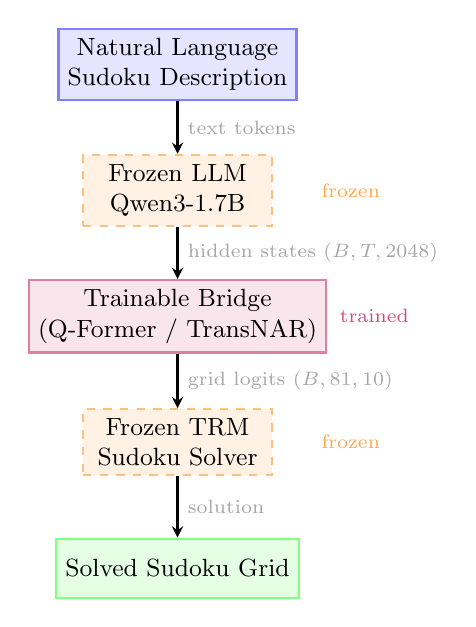
\begin{tikzpicture}[
    box/.style={rectangle, draw, thick, minimum width=2.4cm, minimum height=0.75cm, align=center, font=\small},
    input/.style={box, fill=blue!10, draw=blue!50},
    frozen/.style={box, fill=orange!10, draw=orange!50, dashed},
    bridge/.style={box, fill=purple!10, draw=purple!50},
    output/.style={box, fill=green!10, draw=green!50},
    arrow/.style={->, >=stealth, thick},
    label/.style={font=\scriptsize, color=gray!70}
]

% Nodes
\node[input]  (inp)    at (0,    0) {Natural Language\\Sudoku Description};
\node[frozen] (llm)    at (0,   -1.6) {Frozen LLM\\Qwen3-1.7B};
\node[bridge] (bridge) at (0,   -3.2) {Trainable Bridge\\(Q-Former / TransNAR)};
\node[frozen] (trm)    at (0,   -4.8) {Frozen TRM\\Sudoku Solver};
\node[output] (out)    at (0,   -6.4) {Solved Sudoku Grid};

% Arrows
\draw[arrow] (inp)    -- node[right, label] {text tokens} (llm);
\draw[arrow] (llm)    -- node[right, label] {hidden states $(B,T,2048)$} (bridge);
\draw[arrow] (bridge) -- node[right, label] {grid logits $(B,81,10)$} (trm);
\draw[arrow] (trm)    -- node[right, label] {solution} (out);

% Frozen annotation
\node[label, color=orange!70, align=left] at (2.2, -1.6) {frozen};
\node[label, color=orange!70, align=left] at (2.2, -4.8) {frozen};
\node[label, color=purple!70, align=left] at (2.5, -3.2) {trained};

\end{tikzpicture}
\caption{Pipeline overview. A frozen LLM encodes a natural-language Sudoku description; a trainable bridge maps hidden states to a grid; a frozen TRM solves the puzzle. Only the bridge is trained.}
\label{fig:sudoku_pipeline}
\end{figure}


Many useful large language model (LLM) applications are not pure text generation tasks.
They require a system to interpret a natural-language request and then produce an output that can be checked against formal constraints.
Examples include planning, logical reasoning, and mathematical word problems \cite{gaoPALProgramaidedLanguage2023,panLogicLMEmpoweringLarge2023,kambhampatiLLMsCantPlan2024}.
Prior work on modular and tool-augmented language systems addresses this split by using the LLM as an interface to external tools, programs, or solvers \cite{karpasMRKLSystemsModular2022,parisiTALMToolAugmented2022,gaoPALProgramaidedLanguage2023,panLogicLMEmpoweringLarge2023}.
General-purpose language models struggle to solve these constraint-satisfaction tasks directly through autoregressive text generation.
By contrast, a specialist trained on structured Sudoku grids can focus on the constrained computation.
The Tiny Recursive Model (TRM) solves Sudoku-Extreme puzzles at 86\% exact accuracy with only 5M parameters by iteratively refining a latent state over a fixed number of recursive passes \cite{jolicoeur-martineauLessMoreRecursive2025}.
This suggests a more specific interface problem: fine-tuning a compact language model can teach it to parse natural-language descriptions into structured grids, but not to solve the puzzles directly.
There is also a preservation reason to avoid modifying the LLM: prior work reports that narrow task-specific fine-tuning can degrade domain knowledge, reasoning, and general instruction-following ability \cite{ghoshCloserLookLimitations2024,kalajdzievskiScalingLawsForgetting2024,luoEmpiricalStudyCatastrophic2025}. Section~\ref{sec:llm_frontend_motivation} discusses this risk in more detail.

Figure~\ref{fig:sudoku_pipeline} shows the proposed pipeline: a frozen LLM encodes the natural-language description, a trainable bridge converts the hidden states into grid logits, and a frozen TRM produces the solution.
I connect a frozen Qwen3-1.7B \cite{yangQwen3TechnicalReport2025} to a frozen TRM Sudoku specialist \cite{jolicoeur-martineauLessMoreRecursive2025} through a bridge that maps LLM hidden states to the discrete grid format the specialist expects, keeping both endpoints fixed and concentrating all learning in the bridge.
The design follows the frozen-endpoint bridging approach of BLIP-2 \cite{liBLIP2BootstrappingLanguageImage2023} and TransNAR \cite{bounsiTransformersMeetNeural2024}, applied here to connect an LLM to a learned recursive specialist rather than to a vision encoder or a graph neural network.

This pipeline has the clearest advantage when users describe a task in language, but the computation is better handled in a structured representation than in generated text.
Unlike direct fine-tuning, it does not make the LLM learn the computation itself; unlike tool prompting, it can connect to learned specialists whose interface is not a text API.
This paper evaluates that setting in one controlled task: natural-language Sudoku.

I evaluate four bridge architectures on natural-language Sudoku descriptions generated by two rule-based generators and one LLM-based generator.
The best configuration, a TransNAR bridge trained on structurally noisy descriptions, achieves 86.6\% end-to-end exact solve accuracy, matching the TRM's standalone performance of 86.5\% on these specific test puzzles, while updating only 7.95M parameters, or 0.47\% of the parameters updated by direct Qwen fine-tuning.

This thesis asks one overarching question: can a small trainable bridge connect a frozen LLM to a frozen learned specialist, making the specialist accessible from natural language without modifying either endpoint?

I evaluate this question through four component-level and system-level research questions in Section~\ref{sec:results}:

\begin{description}
    \item[RQ1] Can a small bridge faithfully translate natural-language Sudoku descriptions into structured grid inputs?
    \item[RQ2] Does the frozen TRM specialist solve reliably when given well-formed grid inputs?
    \item[RQ3] Does the full LLM--Bridge--TRM pipeline outperform direct LLM baselines on end-to-end solve accuracy?
    \item[RQ4] Is the modular pipeline more parameter-efficient than fine-tuning an LLM end-to-end?
\end{description}

\section{Related Work}
\label{sec:related_work}

\subsection{Tiny Recursive Models for Algorithmic Reasoning}
\label{sec:tiny_recursive_models}

Small recursive networks have recently shown that iterative refinement over a shared latent state can substitute for scale on verifiable logic reasoning tasks.
The Hierarchical Reasoning Model (HRM) \cite{wangHierarchicalReasoningModel2025} showed that two small recurrent networks operating at different timescales can solve hard combinatorial puzzles such as Sudoku, Maze, and ARC-AGI with only 27M parameters and around 1000 training examples, outperforming much larger LLMs on these tasks.
Building on HRM, the Tiny Recursive Model (TRM) \cite{jolicoeur-martineauLessMoreRecursive2025} simplifies the design to a single two-layer network with tied weights applied recursively.
With only 7M parameters, less than 0.1\% of a standard 7B-parameter LLM, TRM surpasses most LLMs on ARC-AGI benchmarks \cite{cholletARCAGI2NewChallenge2026}.
The core mechanism is iterative refinement over a shared latent state: the same small block is unrolled many times, each pass updating an internal reasoning state $z$ and a predicted output $y$, acting as a latent scratchpad \cite{kohliLoopThinkGeneralize2026}.
The parameter efficiency and strong task-specific accuracy of TRM make it a natural candidate for a frozen specialist solver that an LLM can be trained to interface with.

\subsection{Bridges between Frozen Model Endpoints}
\label{sec:language_to_structure_interfaces}

A challenge in similar hybrid systems is bridging the representation gap between a pretrained LLM and a downstream specialist that expects structured input.
BLIP-2 \cite{liBLIP2BootstrappingLanguageImage2023} addresses this in the vision-language setting by introducing a lightweight Querying Transformer (Q-Former) that connects a frozen image encoder to a frozen LLM, training only the bridge while leaving both specialists intact.
The Q-Former learns a small set of query vectors that cross-attend to the encoder outputs and produce a fixed-length representation consumable by the LLM, demonstrating that a compact trainable bridge can close a large modality gap without touching either frozen endpoint.
TransNAR \cite{bounsiTransformersMeetNeural2024} applies the same principle in the direction relevant to this work: a pretrained Transformer LLM cross-attends to node embeddings from a frozen graph neural network-based neural algorithmic reasoner, allowing the LLM to leverage structured algorithmic computation on CLRS-Text.
LLaVA \cite{liuVisualInstructionTuning2023a} shows that even a simple two-layer MLP projection between a frozen vision encoder and a frozen LLM is competitive with more complex bridges, suggesting that the frozen-endpoint constraint does not require an elaborate interface to be effective.
The bridge proposed in this work follows the same frozen-endpoint design: a trainable module maps hidden states from a frozen LLM to the structured grid format expected by a frozen TRM specialist, keeping both ends fixed and concentrating all learning in the bridge.

\subsection{LLMs and Specialist Solvers for Verifiable Tasks}
\label{sec:recursive_recurrent_reasoning}

Approaches to solving verifiable tasks from natural language span a spectrum from direct LLM generation to tightly coupled hybrid pipelines.
One family of work treats the LLM as part of a larger tool-using system.
These systems route or translate parts of a task to external tools, generated programs, API calls, knowledge sources, reasoning modules, or symbolic solvers \cite{karpasMRKLSystemsModular2022,parisiTALMToolAugmented2022,gaoPALProgramaidedLanguage2023,schickToolformerLanguageModels2023,panLogicLMEmpoweringLarge2023}.
AlphaGeometry \cite{trinhSolvingOlympiadGeometry2024} follows a related hybrid pattern for olympiad geometry.
It pairs a symbolic deduction engine with a fine-tuned large language model (LLM).
The symbolic engine drives proof search and calls the LLM when it needs auxiliary constructions.
Those constructions are proposed as text, so the interface is still generated text rather than a learned hidden-state mapping.
These systems support the general claim that LLM-centered pipelines can benefit from specialist solvers, but they communicate through text, generated code, API calls, or symbolic languages rather than through a learned hidden-state bridge to a frozen neural specialist.
Section~\ref{sec:tiny_recursive_models} discusses TRM as this kind of learned specialist.
Other work integrates specialists inside the language-model family itself.
Branch-Train-Merge \cite{liBranchTrainMergeEmbarrassinglyParallel2022} trains expert LLMs on different domains and merges or ensembles them, while Branch-Train-MiX \cite{sukhbaatarBranchTrainMiXMixingExpert2024} turns asynchronously trained experts into mixture-of-experts layers with token-level routing.
These approaches improve or extend the generalist model itself; in contrast, this work leaves both the LLM and the learned solver frozen and trains only the interface between them.

\subsection{TRM Extensions and Follow-on Work}
\label{sec:follow_ups}

Several works have directly extended or stress-tested TRM since its release.
Tiny Recursive Control \cite{jainTinyRecursiveControl2025} shows the design transfers beyond puzzles to continuous optimal control under strict hardware constraints.
Tiny Autoregressive Recursive Models \cite{raubaTinyAutoregressiveRecursive2026} adapt TRM to autoregressive language models (LMs) and find the recursive architecture fails while simpler baselines succeed, suggesting TRM's gains depend on its original non-autoregressive setup.
Dreamer \cite{knuppDepthRecurrentAttentionMixtures2026} responds by redesigning the recurrent block with depth-aware attention, showing depth-recurrent models can match models two to eight times larger on language reasoning benchmarks.

\subsection{Depth-via-Recursion in Language Models}
\label{sec:depth_recursion_llms}

A parallel line of work applies the same depth-via-recursion principle directly inside large language models.
Universal Transformers \cite{dehghaniUniversalTransformers2019} are the architectural predecessor: they reuse a shared Transformer block across passes to improve general sequence tasks such as translation and language understanding.
\citet{saunshiReasoningLatentThoughts2025} show that the same looping mechanism has a benefit specifically for reasoning: looping a small transformer many times can match a much deeper model on reasoning tasks with far fewer parameters, while memorization tasks see little benefit, and each additional loop implicitly simulates one step of chain-of-thought reasoning.
\citet{kohliLoopThinkGeneralize2026} show that recurrent-depth transformers achieve systematic generalisation to reasoning chains deeper than those seen during training by scaling inference-time recurrence.
These works build iterative depth into the language model itself; this paper instead keeps the recursive specialist frozen and trains a bridge to connect it to a frozen LLM.

\section{Method}
\label{sec:method}

The method combines two building blocks from the related work: lightweight bridges between frozen endpoints \cite{liBLIP2BootstrappingLanguageImage2023,bounsiTransformersMeetNeural2024}, and small recursive specialists for verifiable tasks \cite{jolicoeur-martineauLessMoreRecursive2025}.
In this pipeline, Qwen hidden states are mapped by a trainable bridge into a $9{\times}9$ Sudoku grid, which is then solved by a TRM specialist.
Figure~\ref{fig:sudoku_pipeline} shows this data flow.
I evaluate the pipeline both before and after this handoff: bridge metrics measure the reconstruction accuracy of the input grid, while end-to-end metrics measure the final solved grid returned by the TRM.
The following subsections describe the language inputs, bridge architectures, specialist solver, and domain-adaptation setup.

\begin{figure*}[t]
\centering
\resizebox{\linewidth}{!}{%
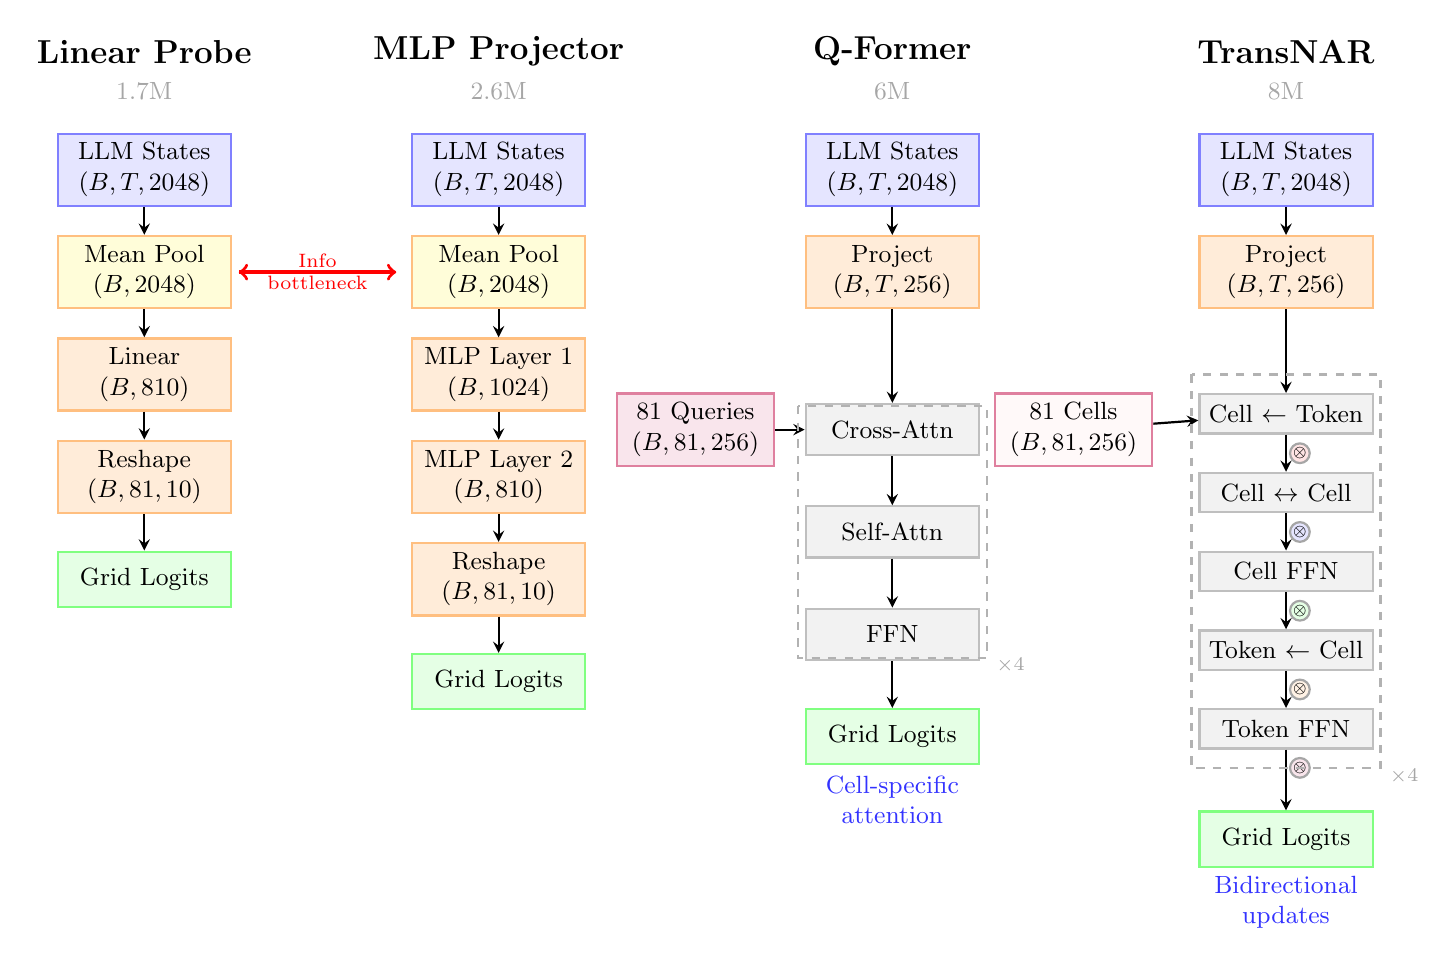
\begin{tikzpicture}[
    box/.style={rectangle, draw, thick, minimum width=2.2cm, minimum height=0.7cm, align=center, font=\small},
    input/.style={box, fill=blue!10, draw=blue!50},
    output/.style={box, fill=green!10, draw=green!50},
    pool/.style={box, fill=yellow!15, draw=orange!50},
    linear/.style={box, fill=orange!15, draw=orange!50},
    query/.style={box, fill=purple!10, draw=purple!50, minimum width=2.0cm},
    attn/.style={box, fill=gray!10, draw=gray!50, minimum height=0.65cm},
    arrow/.style={->, >=stealth, thick},
    title/.style={font=\large\bfseries},
    params/.style={font=\small, color=gray!70}
]

% Architecture 1: Linear Probe
\node[title] at (0, 0) {Linear Probe};
\node[params] at (0, -0.5) {1.7M};
\node[input] (in1) at (0, -1.5) {LLM States\\$(B,T,2048)$};
\node[pool] (pool1) at (0, -2.8) {Mean Pool\\$(B,2048)$};
\node[linear] (lin1) at (0, -4.1) {Linear\\$(B,810)$};
\node[linear] (reshape1) at (0, -5.4) {Reshape\\$(B,81,10)$};
\node[output] (out1) at (0, -6.7) {Grid Logits};
\draw[arrow] (in1) -- (pool1);
\draw[arrow] (pool1) -- (lin1);
\draw[arrow] (lin1) -- (reshape1);
\draw[arrow] (reshape1) -- (out1);
\node[font=\scriptsize, color=red, align=center] at (2.2, -2.8) {Info\\bottleneck};
\draw[->, red, very thick] (1.8, -2.8) -- (1.2, -2.8);
\draw[<-, red, very thick] (3.2, -2.8) -- (1.2, -2.8);

% Architecture 2: MLP Projector
\node[title] at (4.5, 0) {MLP Projector};
\node[params] at (4.5, -0.5) {2.6M};
\node[input] (in2) at (4.5, -1.5) {LLM States\\$(B,T,2048)$};
\node[pool] (pool2) at (4.5, -2.8) {Mean Pool\\$(B,2048)$};
\node[linear] (mlp2a) at (4.5, -4.1) {MLP Layer 1\\$(B,1024)$};
\node[linear] (mlp2b) at (4.5, -5.4) {MLP Layer 2\\$(B,810)$};
\node[linear] (reshape2) at (4.5, -6.7) {Reshape\\$(B,81,10)$};
\node[output] (out2) at (4.5, -8.0) {Grid Logits};
\draw[arrow] (in2) -- (pool2);
\draw[arrow] (pool2) -- (mlp2a);
\draw[arrow] (mlp2a) -- (mlp2b);
\draw[arrow] (mlp2b) -- (reshape2);
\draw[arrow] (reshape2) -- (out2);

% Architecture 3: Q-Former
\node[title] at (9.5, 0) {Q-Former};
\node[params] at (9.5, -0.5) {6M};
\node[input] (in3) at (9.5, -1.5) {LLM States\\$(B,T,2048)$};
\node[linear] (proj3) at (9.5, -2.8) {Project\\$(B,T,256)$};
\node[query] (q3) at (7.0, -4.8) {81 Queries\\$(B,81,256)$};
\node[attn] (cross3) at (9.5, -4.8) {Cross-Attn};
\node[attn] (self3) at (9.5, -6.1) {Self-Attn};
\node[attn] (ffn3) at (9.5, -7.4) {FFN};
\node[output] (out3) at (9.5, -8.7) {Grid Logits};
\draw[arrow] (in3) -- (proj3);
\draw[arrow] (proj3) -- (cross3);
\draw[arrow] (q3) -- (cross3);
\draw[arrow] (cross3) -- (self3);
\draw[arrow] (self3) -- (ffn3);
\draw[arrow] (ffn3) -- (out3);
\draw[dashed, gray!60, thick] (8.3, -4.5) rectangle (10.7, -7.7);
\node[font=\scriptsize, gray!70] at (11.0, -7.8) {$\times$4};
\node[font=\small, color=blue!80, align=center] at (9.5, -9.5) {Cell-specific\\attention};

% Architecture 4: TransNAR
\node[title] at (14.5, 0) {TransNAR};
\node[params] at (14.5, -0.5) {8M};
\node[input] (in4) at (14.5, -1.5) {LLM States\\$(B,T,2048)$};
\node[linear] (proj4) at (14.5, -2.8) {Project\\$(B,T,256)$};
\node[query, fill=pink!10] (cell4) at (11.8, -4.8) {81 Cells\\$(B,81,256)$};
\node[attn, minimum height=0.5cm] (gate4a) at (14.5, -4.6) {Cell $\leftarrow$ Token};
\node[attn, minimum height=0.5cm] (gate4b) at (14.5, -5.6) {Cell $\leftrightarrow$ Cell};
\node[attn, minimum height=0.5cm] (ffn4a) at (14.5, -6.6) {Cell FFN};
\node[attn, minimum height=0.5cm] (gate4c) at (14.5, -7.6) {Token $\leftarrow$ Cell};
\node[attn, minimum height=0.5cm] (ffn4b) at (14.5, -8.6) {Token FFN};
\node[output] (out4) at (14.5, -10.0) {Grid Logits};
\draw[arrow] (in4) -- (proj4);
\draw[arrow] (proj4) -- (gate4a);
\draw[arrow] (cell4) -- (gate4a);
\draw[arrow] (gate4a) -- node[xshift=5pt, circle, fill=red!10, draw=gray!70, inner sep=0pt, minimum size=0.25cm, font=\tiny] {$\otimes$} (gate4b);
\draw[arrow] (gate4b) -- node[xshift=5pt, circle, fill=blue!10, draw=gray!70, inner sep=0pt, minimum size=0.25cm, font=\tiny] {$\otimes$} (ffn4a);
\draw[arrow] (ffn4a) -- node[xshift=5pt, circle, fill=green!10, draw=gray!70, inner sep=0pt, minimum size=0.25cm, font=\tiny] {$\otimes$} (gate4c);
\draw[arrow] (gate4c) -- node[xshift=5pt, circle, fill=orange!10, draw=gray!70, inner sep=0pt, minimum size=0.25cm, font=\tiny] {$\otimes$} (ffn4b);
\draw[arrow] (ffn4b) -- node[pos=0.3, xshift=5pt, circle, fill=purple!10, draw=gray!70, inner sep=0pt, minimum size=0.25cm, font=\tiny] {$\otimes$} (out4);
\draw[dashed, gray!60, thick] (13.3, -4.1) rectangle (15.7, -9.1);
\node[font=\scriptsize, gray!70] at (16.0, -9.2) {$\times$4};
\node[font=\small, color=blue!80, align=center] at (14.5, -10.8) {Bidirectional\\updates};

\end{tikzpicture}%
}
\caption{Comparison of four bridge architectures for mapping LLM hidden states to Sudoku grid predictions. Linear probe and MLP projector pool all tokens into a single vector (information bottleneck), losing cell-specific information. Q-Former uses 81 learnable queries to extract cell-specific features through cross-attention and self-attention. TransNAR extends this with bidirectional gating between token and cell state streams, enabling iterative refinement.}
\label{fig:bridge_architectures}
\end{figure*}


\subsection{Synthetic Language Sudoku Inputs}
\label{sec:synthetic_language_sudoku_inputs}

All puzzles are drawn from the \texttt{sapientinc/sudoku-extreme} dataset \cite{SapientincSudokuextremeDatasets}, the same source used to train the TRM specialist.
I use synthetic descriptions because RQ1 requires paired natural-language inputs and exact grid targets at scale.
The generators keep the underlying puzzle distribution fixed while varying only the language interface.

I use two rule-based generators for training and validation.
The first, `Varied', renders each Sudoku grid as a row-wise text block.
It samples from 5 clue-phrase templates and 5 row orderings to produce controlled surface variation, for example:
\begin{verbatim}
row 1 has 8 in column 4 and 3 in column 9
row 2: column 6 is 5
in row 4, c1=7 and c8=2
\end{verbatim}
The second, `Varied+', tests a noisier language interface.
It draws from 45 layout templates that mix row-wise, column-wise, box-wise, and flat orderings, 12 clue notation formats, and conversational noise tokens.
This produces descriptions that look more like informal transcriptions than structured lists, for example:
\begin{verbatim}
sudoku clues copied from sheet:
by rows:
r3: c2=4 | c5 is 7 | c8=1
by boxes:
Box 2: r1c4=8, r2c6=5
flat clue list:
r7c3=6 -> confirmed
[r7,c6]=2
\end{verbatim}
Both rule-based generators enforce strict validation, so their descriptions are noise-free by construction.

The third source is an LLM-generated set used only for out-of-distribution evaluation.
It tests whether bridges trained on rule-based data transfer to descriptions with less templated phrasing.
Full generator details and validation checks are in Appendix~\ref{app:nl_transformations}.



\subsection{Text-to-Grid Bridge}
\label{sec:text_to_grid_bridge}

The bridge connects the LLM to the TRM specialist by mapping token-level features to structured grid predictions.
A natural-language Sudoku description is tokenized and passed through Qwen \cite{yangQwen3TechnicalReport2025} LLM; hidden states from a chosen layer are extracted as token-wise features of dimension $d_\text{LLM}$, (where $d_\text{LLM} = 2048$ for Qwen3-1.7B).
The bridge maps these features to logits over 81 cells, each predicting one of 10 classes.
To connect the bridge to the TRM, these logits are converted to the specialist's input format by taking the argmax over the 10 class predictions for each of the 81 cells.
Class 0 is decoded as an empty cell, and classes 1--9 are decoded as digits, producing the 81-character puzzle string consumed by the TRM.

I compare four bridge architectures that share this input/output interface but differ in how they aggregate the token sequence into cell predictions (Figure~\ref{fig:bridge_architectures}).
The main contrast in the figure is whether the bridge compresses all token states into one pooled vector before predicting the grid, or keeps separate cell-level states that can attend to the token sequence.
This pooled path is marked as the information bottleneck in Figure~\ref{fig:bridge_architectures}: one vector must contain enough information to predict all 81 cells.
Section~\ref{sec:pipeline_error_sources} later analyses how this bottleneck limits bridge accuracy.

The first pooling-based bridge, the \textbf{linear probe}, applies mean pooling to the token representations $H \in \mathbb{R}^{T \times d_{\text{LLM}}}$ to obtain a single vector $h_{\text{pool}} = \frac{1}{T} \sum_{t=1}^T H_t$, where $T$ represents the sequence length in tokens and $H_t \in \mathbb{R}^{d_{\text{LLM}}}$ is the hidden state vector of the $t$-th token.
It then applies one linear projection $Y = W h_{\text{pool}} + b$ to predict logits $Y \in \mathbb{R}^{81 \times 10}$ for all 81 cells simultaneously.
This serves as a minimal baseline testing linear separability.
The \textbf{MLP projector} adds non-linear capacity by replacing the linear layer with a two-layer multi-layer perceptron (MLP) with GELU activations: $Y = W_2 \text{GELU}(W_1 h_{\text{pool}} + b_1) + b_2$.
The \textbf{Q-Former bridge} \cite{liBLIP2BootstrappingLanguageImage2023} removes the information bottleneck of mean-pooling by using 81 learnable query vectors $Q \in \mathbb{R}^{81 \times d_{\text{bridge}}}$, one for each Sudoku cell.
Each query is combined with a trainable positional table initialized from sinusoidal functions of the cell's row, column, and 3$\times$3 box index.
The box index identifies which of the nine Sudoku subgrids contains the cell, reflecting the third Sudoku constraint in addition to rows and columns.
In Figure~\ref{fig:bridge_architectures}, this is the ``81 Queries'' path leading into cell-specific attention.
Each query represents one grid cell, so the model can align individual cell states with the relevant tokens instead of predicting the whole grid from one pooled vector.
Through $L$ stacked layers, the queries iteratively cross-attend to the projected LLM token states $V = H W_{\text{proj}}$, shown as the token stream in Figure~\ref{fig:bridge_architectures}.
They then update through self-attention and a feed-forward network (FFN), while keeping token states fixed.
Cross-attention lets each cell query read the language-model tokens.
Self-attention lets the 81 cell states exchange information before classification.
This is useful because Sudoku cells are coupled by row, column, and 3$\times$3 box constraints, and because descriptions often group clues by these structures.
A final linear classifier maps each query to 10 class logits.
The \textbf{TransNAR bridge} \cite{bounsiTransformersMeetNeural2024} keeps the same 81 cell states as Q-Former, but also updates the projected token states.
This makes the bridge bidirectional.
Cells can read from the language representation, and the language-token stream can later be refined using the current cell states.
The TransNAR column in Figure~\ref{fig:bridge_architectures} shows one repeated block.
First, ``Cell $\leftarrow$ Token'' is cross-attention from the 81 cell states to the projected token states.
Next, ``Cell $\leftrightarrow$ Cell'' is self-attention among the cell states, letting cells exchange row, column, and box information.
The cell FFN then updates the cell stream.
The final two blocks implement the reverse direction: tokens read back from cells, and a token FFN updates the token stream.
Each update is modulated by a learnable scalar gate $g$ initialized to zero and passed through a $\tanh$ activation:
\begin{equation}
x_{\text{new}} = x_{\text{old}} + \tanh(g) \cdot \text{Sublayer}(x_{\text{old}})
\end{equation}
This gating mechanism ensures the bridge starts as an identity function and safely integrates bidirectional information without destabilizing early training.
As shown in Figure~\ref{fig:bridge_architectures}, Q-Former and TransNAR both read from projected LLM token states because the Qwen hidden dimension is larger than the bridge dimension.
The projection keeps the bridge lightweight, but it is also a compression step: information not preserved in $V = H W_{\text{proj}}$ cannot be recovered by later attention layers.
The target input grids are sparse: most cells are empty, while only the starting clue cells contain digits.
Without class weighting, a bridge can obtain a high cell-level score by over-predicting empty cells.
All four bridges are therefore trained with cross-entropy loss, with a higher class weight on digit classes relative to empty cells.
\subsection{TRM Sudoku Solver}
\label{sec:trm_specialist}

The Tiny Recursive Model (TRM) \cite{jolicoeur-martineauLessMoreRecursive2025} is a recurrent neural network that solves constraint-satisfaction tasks through depth-wise parameter sharing.
Rather than stacking distinct layers, a TRM unrolls a single lightweight reasoning block over a fixed number of recursive passes, allowing it to perform deep computation with a very small parameter footprint.

To process a puzzle, an embedding layer maps each cell integer of the input grid to a vector representation, forming the initial cell states.
At each recursive step, a shared block updates the cell representations.
Because the weights of this block are shared across all steps, the model can scale its computational depth without increasing its parameter budget.
To optimize performance on the small, fixed Sudoku grid, the Sudoku specialist TRM checkpoint replaces self-attention with a spatial Multilayer Perceptron (MLP) block inspired by the MLP-Mixer architecture.
This block consists of a token-mixing MLP (which mixes information across cell positions to propagate row, column, and box constraints) and a channel-mixing MLP (which mixes information across the feature channels of each cell representation).
This unrolling of the shared token- and channel-mixing MLPs allows the model to iteratively propagate constraints across the entire grid in the latent space.
After the final pass, a classification head projects the cell states to produce the solved digit predictions.

In this work, I train a 5M-parameter TRM Sudoku solver using the implementation provided by \citet{jolicoeur-martineauLessMoreRecursive2025}.
Almost all parameters belong to the recurrent reasoning core rather than the vocabulary tables: the model contains 5.03M learned parameters, of which only 6.1K (0.12\%) are input or puzzle embeddings, leaving 5.02M non-embedding parameters.
Its weights are frozen throughout all subsequent bridge experiments.


\subsection{Adapting to a New Specialist Interface}
\label{sec:domain_adaptation}

The same frozen-endpoint design can be ported to another specialist interface by changing the paired data and the decoder into the specialist's native input format.
For Sudoku, the bridge target is a $9{\times}9$ grid.
For a CLRS-style algorithmic specialist, the bridge target is a set of native input tensors such as node masks, edge matrices, scalar arrays, and pointer-like fields.
The shared requirement is that each natural-language example has an exact structured target, so bridge errors can be measured before the specialist is run.
This paper uses Sudoku as the main benchmark and includes a smaller CLRS input-reconstruction text study as a preliminary check that the bridge setup can connect to another family of specialists.

\section{Data and Experimental Design}
\label{sec:experiments}
\label{sec:training_setup}

I keep the Qwen3-1.7B \cite{yangQwen3TechnicalReport2025} LLM and TRM specialist fixed across bridge runs.
This isolates the effect of the bridge architecture and makes the comparison with direct LLM fine-tuning clear.
The bridge variants are a linear probe, an MLP projector, Q-Former, and TransNAR.
The end-to-end baselines are direct Qwen3-1.7B fine-tuning and frontier-model zero-shot prompting.

\paragraph{Data splits.}
The 10,000-example Varied and Varied+ datasets are each split 80/10/10 into train, validation, and test sets.
A separate 1,000-example LLM-generated set is held out entirely as an out-of-distribution test.
This set measures whether bridges trained on rule-based descriptions transfer to more natural phrasing produced by an LLM (see Appendix~\ref{app:llm_model_selection} and~\ref{app:llm_nl_generation}).

\paragraph{Data validation.}
I validate each generated description by parsing it back into a Sudoku grid.
The Varied and Varied+ rule-based generators construct descriptions directly from the source puzzle, so the generated text is designed to preserve the original grid.
The parser check confirms that the generated description recovers the same grid.
For the LLM-generated test set, I use the same parser to measure how often the text preserves the intended puzzle.
Appendix~\ref{app:llm_nl_generation} reports those validation results.

\paragraph{Training details.}
All bridge and fine-tuning hyperparameters are listed in Appendix~\ref{app:hyperparameters}.

\section{Results}
\label{sec:results}

The following subsections address each research question in turn using the experimental conditions described above, followed by a preliminary CLRS input-reconstruction text study.

\subsection*{Research Question 1}
\label{sec:bridge_performance}

\paragraph{Can a Small Bridge Faithfully Translate Natural-Language Sudoku Descriptions into Structured Grid Inputs?}
I evaluate whether each bridge can reconstruct the input grid from a natural-language Sudoku description.
Cell accuracy measures correctness over the 81 grid positions, while exact grid match requires all 81 cells to be correct.

\begin{table*}[t]
\centering
\caption{Bridge text-to-grid accuracy for systems trained on the Varied 10K dataset. Varied test is the held-out Varied test set; LLM (OOD) is the LLM-generated held-out set. Metrics are percentages. Dashes mark metrics or conditions unavailable for this training distribution. Bold indicates the best reported result per column.}
\label{tab:bridge_varied}
\begin{tabular}{lcccc}
\toprule
& \multicolumn{2}{c}{Varied test} & \multicolumn{2}{c}{LLM (OOD)} \\
\cmidrule(lr){2-3}\cmidrule(lr){4-5}
System & Cell acc. (\%) & Exact (\%) & Cell acc. (\%) & Exact (\%) \\
\midrule
\multicolumn{5}{l}{\textit{Zero-shot}} \\
\midrule
DeepSeek-V4-Pro (no CI)$^\dagger$ & 61.4 & 0.0 & 62.6 & 0.0 \\
\midrule
\multicolumn{5}{l}{\textit{Autoregressive fine-tuning}} \\
\midrule
Qwen3-1.7B FT (grid)          & 98.9 & 96.6 & 70.1 & 0.2 \\
\midrule
\multicolumn{5}{l}{\textit{Trainable bridges}} \\
\midrule
Linear probe  & 65.1 & 0.0 & 52.5 & 0.0 \\
MLP projector & 68.9 & 0.0 & 68.8 & 0.0 \\
Q-Former      & 96.8 & 4.3 & 96.9 & 4.4 \\
TransNAR      & \textbf{100.0} & \textbf{99.3} & \textbf{98.4} & \textbf{29.7} \\
\bottomrule
\end{tabular}

\vspace{0.5em}
\noindent\small $^\dagger$ Run without reasoning (enabling reasoning caused infinite generation loops without yielding a final result).
\end{table*}

\begin{table*}[!t]
\centering
\caption{Bridge text-to-grid accuracy for systems trained on the Varied+ 10K dataset. Varied+ test is the held-out Varied+ test set; LLM (OOD) is the LLM-generated held-out set. Metrics are percentages. Dashes mark unavailable metrics. Bold indicates the best result per column.}
\label{tab:bridge_variedplus}
\begin{tabular}{lcccc}
\toprule
& \multicolumn{2}{c}{Varied+ test} & \multicolumn{2}{c}{LLM (OOD)} \\
\cmidrule(lr){2-3}\cmidrule(lr){4-5}
System & Cell acc. (\%) & Exact (\%) & Cell acc. (\%) & Exact (\%) \\
\midrule
\multicolumn{5}{l}{\textit{Zero-shot}} \\
\midrule
DeepSeek-V4-Pro (no CI)$^\dagger$ & 58.2 & 0.0 & 62.6 & 0.0 \\
\midrule
\multicolumn{5}{l}{\textit{Autoregressive fine-tuning}} \\
\midrule
Qwen3-1.7B FT (grid)          & 97.3 & 90.9 & 98.0 & 93.3 \\
\midrule
\multicolumn{5}{l}{\textit{Trainable bridges}} \\
\midrule
Linear probe  & 68.6 & 0.0 & 35.5 & 0.0 \\
MLP projector & 68.9 & 0.0 & 66.8 & 0.0 \\
Q-Former      & 99.8 & 90.2 & 99.9 & 95.0 \\
TransNAR      & \textbf{100.0} & \textbf{98.3} & \textbf{100.0} & \textbf{99.3} \\
\bottomrule
\end{tabular}

\vspace{0.5em}
\noindent\small $^\dagger$ Run without reasoning (enabling reasoning caused infinite generation loops without yielding a final result).
\end{table*}

\begin{table*}[!t]
\centering
\caption{End-to-end exact solve accuracy. Varied+ = rule-based Varied+ test set (1,000 examples); OOD = LLM-generated out-of-distribution set. $n$ = number of examples evaluated. Metrics are percentages. Dashes indicate the condition was not evaluated. CI = code interpreter.}
\label{tab:e2e_results}
\begin{tabular}{llccc}
\toprule
System & Variant & $n$ & Varied+ exact (\%) & OOD exact (\%) \\
\midrule
\multicolumn{5}{l}{\textit{Zero-shot}} \\
\midrule
Qwen3-1.7B                      & zero-shot           & 1000 & 0.0 & 0.0 \\
DeepSeek-V4-Pro (no CI)$^\dagger$ & zero-shot           & 25   & 0.0 & 0.0 \\
\midrule
\multicolumn{5}{l}{\textit{End-to-end fine-tuning}} \\
\midrule
Qwen3-1.7B FT                   & Varied              & 1000 & 0.0 & 0.0 \\
Qwen3-1.7B FT                   & Varied+             & 1000 & 0.1 & 0.3 \\
\midrule
\multicolumn{5}{l}{\textit{Bridge + TRM specialist}} \\
\midrule
Qwen3-1.7B FT$^\ddagger$        & Varied              & 1000 & 0.5 & 0.1 \\
Q-Former                 & Varied              & 1000 & 0.0 & 9.6 \\
TransNAR                 & Varied              & 1000 & 0.5 & 33.9 \\
Qwen3-1.7B FT$^\ddagger$        & Varied+             & 1000 & 77.5 & 79.3 \\
Q-Former                 & Varied+             & 1000 & 79.3 & 79.9 \\
\textbf{TransNAR}                 & \textbf{Varied+}             & \textbf{1000} & \textbf{86.6} & \textbf{85.5} \\
\bottomrule
\end{tabular}

\vspace{0.5em}
\noindent\small $^\dagger$ Run without reasoning (enabling reasoning caused infinite generation loops without yielding a final result).

\noindent\small $^\ddagger$ Qwen3-1.7B fine-tuned to generate the initial puzzle grid autoregressively; TRM then solves from that grid.
\end{table*}

Tables~\ref{tab:bridge_varied} and~\ref{tab:bridge_variedplus} report results for bridges trained on the Varied and Varied+ datasets respectively, including a fine-tuned Qwen3-1.7B baseline that generates the grid autoregressively rather than through a bridge.
The linear probe and MLP projector fail under both training distributions: in Table~\ref{tab:bridge_varied}, exact grid match is 0.0\% for both, and in Table~\ref{tab:bridge_variedplus}, exact grid match is also 0.0\% for both.
Their cell accuracy stays close to the empty-cell baseline, around 65--69\% in Table~\ref{tab:bridge_varied} and 69\% for the Varied+ test column in Table~\ref{tab:bridge_variedplus}, consistent with collapsing toward predicting empty cells.
On the Varied test set in Table~\ref{tab:bridge_varied}, Q-Former reaches 4.3\% exact grid match while TransNAR reaches 99.3\%.
However, the LLM (OOD) columns in Table~\ref{tab:bridge_varied} show poor transfer from Varied training: TransNAR reaches 29.7\% exact grid match, Q-Former reaches 4.4\%, and Qwen3-1.7B FT reaches 0.2\%.
This shows that the fixed sentence structure of Varied limits transfer to inputs with different phrasing.
To test whether noisier natural-language transformations improve robustness, I continued training on Varied+.
In Table~\ref{tab:bridge_variedplus}, TransNAR reaches 98.3\% exact grid match on the Varied+ test set and 99.3\% on the LLM out-of-distribution set.
The same table shows Q-Former at 90.2\% and 95.0\% exact grid match, and Qwen3-1.7B FT at 90.9\% and 93.3\%.
Overall, Table~\ref{tab:bridge_variedplus} shows that TransNAR trained on Varied+ reaches the highest exact match on both in-distribution and out-of-distribution inputs.

\subsection*{Research Question 2}
\label{sec:standalone_trm_results}

\paragraph{Does the TRM Specialist Solve Reliably When Given Well-Formed Grid Inputs?}
To establish the solver's standalone performance, I evaluate the TRM specialist directly on native $9{\times}9$ integer grid inputs, bypassing the bridge entirely.
Exact match is the fraction of puzzles solved with zero errors, while cell-level accuracy is the fraction of solution cells predicted correctly.
This isolates solver capability from any language parsing errors introduced upstream.

On the 1,000 puzzles used in the pipeline test sets, the checkpoint achieves 86.5\% exact puzzle accuracy and 95.0\% cell-level accuracy.
This differs slightly from the 86.1\% exact accuracy and 94.8\% cell-level accuracy reported in the original TRM paper because the puzzle samples are different \cite{jolicoeur-martineauLessMoreRecursive2025}.

These numbers provide the reference point for interpreting the full pipeline.
When the bridge gives TRM the correct input grid but TRM still fails, the error is a solver failure.
When the bridge gives TRM an incorrect grid, the error is an interface failure.

\subsection*{Research Question 3}
\label{sec:end_to_end_pipeline_results}

\paragraph{Does the Full LLM--Bridge--TRM Pipeline Outperform Direct LLM Baselines on End-to-End Solve Accuracy?}
End-to-end exact solve accuracy is the fraction of puzzles where the final solved grid is fully correct.
Table~\ref{tab:e2e_results} summarises this metric across all systems evaluated on the Varied+ test set (1,000 examples) and the LLM-generated out-of-distribution set.

\paragraph{Direct LLM baselines.}
Qwen3-1.7B zero-shot produces valid output on only 3 of 1,000 examples and achieves 0\% exact solve accuracy, confirming that the base model has no reliable Sudoku-solving capability without task-specific training.
Similarly, zero-shot prompting of DeepSeek-V4-Pro (run without reasoning to avoid infinite generation loops) achieves 0\% exact solve accuracy on a 25-example sample (Table~\ref{tab:e2e_results}).
Fine-tuning Qwen3-1.7B to generate the grid directly (rather than a solved puzzle) reaches 96.6\% exact grid match on Varied and 90.9\% on Varied+ (Tables~\ref{tab:bridge_varied} and~\ref{tab:bridge_variedplus}).
When this grid output is fed into the TRM specialist, the resulting pipeline achieves 82.5\% end-to-end exact solve accuracy on the Varied test set, 77.5\% on Varied+, and 79.3\% on the OOD set.
Fine-tuning Qwen3-1.7B to generate the full solved puzzle directly yields 0\% exact solve accuracy on the Varied validation set and 0.1\% on Varied+, indicating that the model learns surface formatting without learning to solve the puzzle.

\paragraph{Pipeline results.}
The best pipeline configuration, a TransNAR bridge trained on the Varied+ 10K dataset connected to the TRM specialist, achieves 86.6\% exact solve accuracy and 95.0\% cell-level accuracy on 1,000 Varied+ test examples.
This is a substantial improvement over all direct LLM baselines evaluated here.
This effectively matches the TRM's standalone performance of 86.5\% on these specific held-out puzzles (Section~\ref{sec:standalone_trm_results}), and the remaining failures are analysed by bridge and solver source in Section~\ref{sec:pipeline_error_sources}.
When the bridge is not trained on the target distribution (the Varied bridge rows in Table~\ref{tab:e2e_results}), OOD exact solve accuracy drops to 9.6\% for Q-Former and 33.9\% for TransNAR, confirming that bridge quality is the primary bottleneck in the pipeline.

\paragraph{Summary.}
The modular pipeline outperforms the direct LLM baselines evaluated in this section.
The closest direct alternative is Qwen FT (grid) + TRM, which uses a fine-tuned LLM as a grid parser before the same specialist.
It still trails the TransNAR bridge while requiring full-model adaptation.
Directly fine-tuning Qwen to solve puzzles is not competitive.
Section~\ref{sec:recursive_specialization_help} compares the pipeline with GPT-5.4 using tool/code access.

\subsection*{Research Question 4}
\label{sec:efficiency}
\label{sec:efficiency_results}

\paragraph{Is the Modular Pipeline More Efficient Than Fine-Tuning an LLM End-to-End?}
Efficiency in machine-learning experiments is normally reported together with task performance, using quantities such as trainable parameters, runtime, GPU-hours, energy, carbon, and FLOPs \cite{schwartzGreenAI2020,JMLR:v21:20-312}.
In this paper, I evaluate efficiency through adaptation cost: how many parameters are updated to adapt the system to natural-language Sudoku.\footnote{I do not report electricity or FLOP results because the training logs do not record GPU power draw, energy use, or the token and operation counts needed for a defensible estimate.}
I focus on parameter accounting for the specialists and the adaptation surface required to connect them, with the frozen LLM providing a further inference advantage.

Since the bridge-based pipeline matches or outperforms the fine-tuning baselines, the key efficiency comparison is the adaptation cost: the parameter footprint that must be updated to achieve competitive task performance.

I first compare parameter efficiency using the share of parameters allocated to token embeddings.
Scaling-law work commonly defines model size in terms of non-embedding parameters, excluding vocabulary and positional embeddings, because this produces cleaner trends for language-model performance \cite{kaplanScalingLawsNeural2020}.
Under this accounting, a large fraction of small edge-oriented LLMs is spent on token embeddings: Gemma 3 270M allocates 63.0\% of its parameters to embeddings \cite{IntroducingGemma3}; LFM2.5-350M allocates 18.9\% to embeddings because of its 65,536-token tied vocabulary \cite{LFM25350MNoSize,LiquidAILFM25350MHugging2026}; and Qwen3-1.7B, the LLM used in this project, allocates approximately 17.6\% to embeddings \cite{yangQwen3TechnicalReport2025,QwenQwen317BHugging2025}.

\begin{table}[!t]
\centering
\footnotesize
\caption{Effective-parameter comparison. Embedding share is the percentage of total parameters allocated to vocabulary-dependent embedding tables. Gemma and LFM2.5 are included as compact edge-language references; Qwen3-1.7B is the LLM used in this project; TRM is the Sudoku specialist.}
\label{tab:effective_parameter_accounting}
\begin{tabular}{@{}lrr@{}}
\toprule
Model & Params & Embedding share (\%) \\
\midrule
Gemma 3 270M & 270M & 63.0 \\
LFM2.5-350M & 354.5M & 18.9 \\
Qwen3-1.7B & 1.7B & $\sim$17.6 \\
\textbf{TRM Sudoku} & \textbf{5.03M} & \textbf{0.12} \\
\bottomrule
\end{tabular}
\end{table}

Table~\ref{tab:effective_parameter_accounting} shows that the Sudoku TRM allocates only 0.12\% of its parameters to embeddings.
This is the opposite allocation from compact LLMs, where a large vocabulary and language interface consume a substantial share of the total parameter budget before any task-specific reasoning is considered.
The pipeline therefore avoids fine-tuning the 1.7B-parameter LLM end-to-end and instead trains only the bridge while keeping the LLM and 5.03M-parameter recursive specialist fixed.

\begin{table}[!t]
\centering
\scriptsize
\setlength{\tabcolsep}{2pt}
\caption{Adaptation-efficiency comparison. Updated parameters receive gradients during task adaptation. Grid exact is Varied+ held-out test reconstruction. End-to-end exact reports Varied+ / OOD after TRM. Metrics are percentages except parameter counts.}
\label{tab:adaptation_efficiency}
\begin{tabular}{@{}lrrrr@{}}
\toprule
System & Params & Share (\%) & Grid (\%) & E2E (\%) \\
\midrule

Qwen FT + TRM  & 1.7B & 100.00 & 90.9 & 77.5 / 79.3 \\
TransNAR + TRM & 7.95M & 0.47 & 98.3 & 86.6 / 85.5 \\
\bottomrule
\end{tabular}
\end{table}

Table~\ref{tab:adaptation_efficiency} shows that the TransNAR bridge updates 7.95M parameters, or 0.47\% of the parameters updated by full Qwen fine-tuning, while matching or exceeding fine-tuned Qwen on grid reconstruction.
The efficiency result is therefore not an accuracy claim alone: the bridge achieves comparable or better grid reconstruction than fine-tuned Qwen at a fraction of the adaptation cost, while achieving higher end-to-end solve accuracy when connected to the TRM specialist.

\subsection*{Preliminary Study: Does the Bridge Setup Transfer to CLRS Specialists?}
\label{sec:clrs_preliminary_results}

I include a small CLRS input-reconstruction text study to test whether the same bridge idea can attach an LLM to a different specialist family.
This is not a second full benchmark.
It is a preliminary interface experiment: one TransNAR bridge reconstructs native CLRS input tensors from natural-language descriptions, and the algorithm label is used to route each example to the matching single-task M-ReNAR specialist. Each evaluated task uses 200 length-64 level-4 test examples.
The route is provided by the evaluation harness; no learned router is evaluated.

\begin{table*}[t]
\centering
\small
\caption{Preliminary CLRS input-reconstruction text results. One TransNAR bridge is shared across tasks. Routed ReNAR uses the algorithm label to select the single-task M-ReNAR specialist. Bridge row exact is input-tensor exact match with tolerance 0.05 for continuous fields. Native ReNAR is the specialist score on native inputs and serves as an upper-bound control. Metrics are percentages.}
\label{tab:clrs_preliminary_results}
\begin{tabular}{lrrrr}
\toprule
Algorithm & $n$ & Bridge row exact & Native ReNAR & Bridge+routed ReNAR \\
\midrule
\texttt{bfs}                  & 200 & 54.0  & 100.00 & 81.38 \\
\texttt{dfs}                  & 200 & 100.0 & 83.89  & 79.02 \\
\texttt{bellman\_ford}        & 200 & 57.5  & 91.50  & 63.49 \\
\texttt{dijkstra}             & 200 & 52.5  & 96.83  & 66.47 \\
\texttt{dag\_shortest\_paths} & 200 & 52.0  & 89.99  & 70.31 \\
\texttt{binary\_search}       & 200 & 66.5  & 74.95  & 22.50 \\
\texttt{insertion\_sort}      & 200 & 100.0 & 87.26  & 86.41 \\
\bottomrule
\end{tabular}
\end{table*}

Table~\ref{tab:clrs_preliminary_results} shows that the bridge can supply useful native inputs to several CLRS specialists.
The native ReNAR column should be read as an upper-bound control rather than a sample-matched benchmark, because it measures the specialists when native inputs are provided directly.
One illustrative case is \texttt{insertion\_sort}: the bridge reconstructs the input exactly, and the end-to-end score nearly matches the native ReNAR specialist.
For graph tasks, the bridge reconstructs the structural tensors but often misses the source node, so end-to-end performance falls below the native specialist's standalone performance while still retaining part of the specialist's output accuracy.
The \texttt{binary\_search} row is a negative case and is analysed in Section~\ref{sec:clrs_preliminary_analysis}.
These results show that the bridge setup can be reused outside Sudoku, but stronger claims would require a larger CLRS evaluation with matched baselines, learned routing, and a deeper error analysis.

\section{Analysis}
\label{sec:analysis}
\label{sec:pipeline_error_sources}

By separating the evaluation into component-level metrics (the translation accuracy of the bridge in RQ1 and the standalone reliability of the solver in RQ2) and system-level metrics (the end-to-end solve rate in RQ3), I can isolate how errors propagate and compound. The system-level end-to-end accuracy numbers in Table~\ref{tab:e2e_results} combine these two independent component-level failure sources: the bridge may produce an incorrect grid, and the TRM solver may fail even when the bridge is correct.
Separating these two sources matters because they have different remedies: bridge-side failures call for better training data or a more expressive architecture, while solver-side failures reflect the TRM's own accuracy limits.
I run all four bridge architectures on three test sets (Varied, Varied+, and LLM out-of-distribution) and record per-puzzle bridge predictions and TRM predictions, giving a full breakdown of where each failure occurs.
Full per-configuration results are in Tables~\ref{tab:app_bridge_full} and~\ref{tab:app_trm_full} in Appendix~\ref{app:full_pipeline_results}.

The analysis proceeds in three steps.
First, I isolate bridge-side errors: pooling-based bridges collapse to all-empty grids, while attention-based bridges make sparse cell-level mistakes with some row concentration.
I then check whether those failures come from unusable LLM states.
Second, I separate solver errors from interface errors: TRM has a stable standalone accuracy, its failures are global, and it can recover from some bridge mistakes.
Third, I inspect the trained TransNAR gates to see how the best bridge moves information between token and cell states.

\paragraph{Linear and MLP bridges collapse to predicting all-empty.}
Neither the linear probe nor the MLP projector learns to predict given cells.
The MLP predicts all-empty on 99\% of puzzles regardless of training distribution; the linear probe is slightly less degenerate but achieves a given-cell accuracy of under 1\%.
The reported cell accuracy of approximately 69\% for both architectures is entirely explained by the fraction of empty cells in the test puzzles: 68.9\% of all 81 cells are empty, so predicting everything as empty yields that score without recovering a single given.
This confirms that mean-pooling the token sequence into a single vector discards the positional information needed to assign digits to specific cells, and that adding a non-linear layer does not recover it.
The TRM receives an all-empty grid and produces a random-looking output, giving 0\% end-to-end accuracy across all conditions.

\paragraph{Q-Former and TransNAR fail on isolated cells, not whole puzzles.}
When the attention-based bridges fail, they fail on one or two cells.
For the best-performing configuration (TransNAR trained on Varied+, tested on Varied+), 15 of 17 bridge failures involve exactly one wrong cell, and the mean error count across all failures is 1.1 cells.
Q-Former failures are similarly sparse: mean 1.2--2.0 wrong cells depending on the test set.
This is a qualitatively different failure mode from the linear and MLP collapse: the bridge has learned the task and is nearly correct, but occasionally misreads or drops a single clue.

\paragraph{Bridge failures concentrate in specific rows.}
Attention-based bridges fail on isolated cells rather than whole puzzles, and the failures are not uniformly distributed.
For Q-Former on the Varied+ test set, rows 7--9 account for 44\% of all bridge errors despite containing only 33\% of cells.
This row-skew is consistent with the truncation behaviour described in Appendix~\ref{app:sequence_length}: the Varied+ format is verbose, and clues for later rows appear later in the token sequence, where truncation is more likely to cut them off.
This does not show that truncation affects only Q-Former.
Rather, Q-Former produces enough errors for the late-row skew to be visible, while TransNAR makes too few errors on the same split to support a reliable row-level pattern (19 total errors across 17 failures).
Its errors are spread across rows 2--7 with no strong concentration.

\paragraph{LLM hidden states are not the primary failure source.}
One concern is that the LLM produces hidden states too noisy or uninformative for the bridge to recover the correct grid, independent of bridge capacity.
The OOD results argue against this: both Q-Former and TransNAR achieve higher bridge exact match on the LLM out-of-distribution set (95.0\% and 99.3\%) than on the Varied+ in-distribution set (90.2\% and 98.3\%).
If hidden state quality were the bottleneck, OOD performance would be expected to degrade, since OOD inputs are further from the bridge's training distribution and any degradation in the LLM's encoding of puzzle structure would compound with the bridge's reduced familiarity with the input style.
The opposite pattern holds, which suggests the LLM encodes sufficient information for the bridge to extract the grid under both conditions, and that residual bridge failures reflect the bridge's own capacity rather than information loss in the frozen LLM.

\paragraph{The TRM solver performance limits are consistent at 85--87\%.}
Across all five configurations where the bridge achieves high accuracy, the fraction of puzzles that TRM solves given a perfect bridge input falls in the range 83.7--87.1\%, tightly clustered around the 86.5\% standalone exact puzzle solve rate reported in Section~\ref{sec:standalone_trm_results}.
This confirms that this standalone solve rate is a property of the checkpoint, not of the pipeline or the test set.
Any end-to-end accuracy shortfall below this baseline is attributable to bridge errors.

\paragraph{TRM failures are global, not local.}
Unlike bridges, which only fail on isolated cells, TRM fails globally: when the solver misses a puzzle on a perfect bridge input, it typically gets approximately 30 cells wrong (mean 29.9 for TransNAR Varied+/Varied+).
The errors are distributed uniformly across all 81 cells with no spatial pattern, which is consistent with a global constraint-satisfaction failure. Because cell values are highly interdependent in Sudoku, any local error propagates through the row, column, and block constraint paths during the solver's recursive updates. Consequently, the model's recurrent dynamics do not settle on a grid with a single localized error; instead, the iterative refinement converges to a stable but incorrect grid configuration (a fixed point of the recurrence relation) where many cell predictions are corrupted simultaneously.
Puzzle difficulty predicts TRM failure: puzzles rated 0 (trivially easy) have a 0\% TRM failure rate, while puzzles rated 1--40 fail at 10--21\%.
The strongest single predictor is the number of empty cells: puzzles with 54 or fewer empty cells have 0\% TRM failure, while puzzles with 55--59 empty cells fail at 15.6\%.
This is consistent with the solver's design: more empty cells mean a larger search space, and the fixed number of recursive passes may be insufficient for the hardest instances.

% TRM error recovery 2x2 contingency matrix
% TransNAR Varied+/Varied+, n=1000
\begin{figure}[!t]
\centering
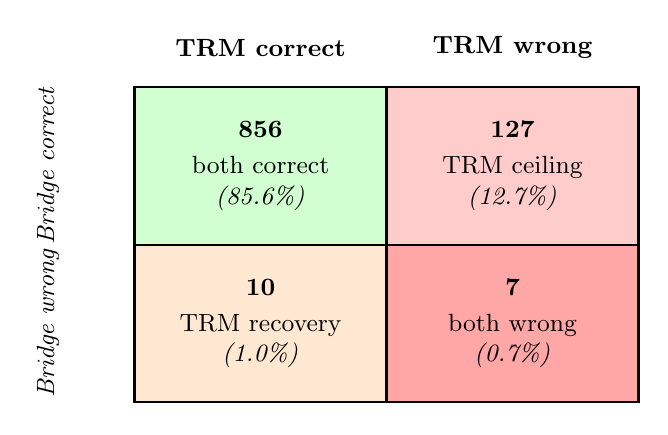
\begin{tikzpicture}[
    cell/.style={
        rectangle,
        draw=black,
        minimum width=3.2cm,
        minimum height=2.0cm,
        align=center,
        font=\small
    },
    header/.style={
        font=\small\bfseries,
        align=center
    },
    axislabel/.style={
        font=\small\itshape,
        align=center
    }
]

% Column headers
\node[header] at (1.6, 0.5)  {TRM correct};
\node[header] at (4.8, 0.5)  {TRM wrong};

% Row headers (rotated)
\node[axislabel, rotate=90] at (-1.1, -1.0) {Bridge correct};
\node[axislabel, rotate=90] at (-1.1, -3.0) {Bridge wrong};

% Top-left: B+T+ (856) -- both correct, lightest fill
\node[cell, fill=green!18] at (1.6, -1.0) {
    \textbf{856}\\[2pt]
    both correct\\
    \textit{(85.6\%)}
};

% Top-right: B+T- (127) -- bridge ok, TRM fails, medium fill
\node[cell, fill=red!20] at (4.8, -1.0) {
    \textbf{127}\\[2pt]
    TRM ceiling\\
    \textit{(12.7\%)}
};

% Bottom-left: B-T+ (10) -- bridge fails, TRM recovers, light fill
\node[cell, fill=orange!18] at (1.6, -3.0) {
    \textbf{10}\\[2pt]
    TRM recovery\\
    \textit{(1.0\%)}
};

% Bottom-right: B-T- (7) -- both fail, darkest fill
\node[cell, fill=red!35] at (4.8, -3.0) {
    \textbf{7}\\[2pt]
    both wrong\\
    \textit{(0.7\%)}
};

% Outer border
\draw[thick] (0, 0) rectangle (6.4, -4.0);
% Inner dividers
\draw[thick] (3.2, 0) -- (3.2, -4.0);
\draw[thick] (0, -2.0) -- (6.4, -2.0);

\end{tikzpicture}
\caption{Outcome breakdown for the TransNAR bridge trained on Varied+ data and evaluated on the Varied+ test set ($n=1000$). Rows indicate whether the bridge produced a correct grid; columns indicate whether TRM produced a correct solution. The dominant failure mode is B$^+$T$^-$: the bridge is correct but TRM fails, reflecting the solver's own accuracy ceiling. B$^-$T$^+$ cases (TRM recovers despite a bridge error) are rare and are analysed in the text.}
\label{fig:trm_recovery_matrix}
\end{figure}


\paragraph{TRM error recovery depends on the type of bridge error.}
For the best-performing pipeline on the Varied+ test set (TransNAR bridge trained on Varied+ data, 86.6\% end-to-end exact solve), 856 of 1,000 puzzles have both bridge and TRM correct, 127 have a correct bridge but a wrong TRM output, 10 have a wrong bridge but a correct TRM output, and 7 have both wrong (Figure~\ref{fig:trm_recovery_matrix}).
The 127 cases where the bridge is correct but TRM fails represent the solver's own performance limits: puzzles the checkpoint cannot solve regardless of how the input is delivered.

The 10 in-distribution recovery cases all involve the bridge dropping a starting clue cell to empty.
TRM inferred the missing value from the surrounding constraints in every case, and recovered from no case where the bridge predicted a wrong digit instead.
A missing starting clue leaves the constraint system underdetermined but consistent; a wrong digit introduces a contradiction that iterative refinement cannot resolve.

\paragraph{Internal bridge dynamics reveal a write-once token stream.}
Inspecting the trained gate values for the best-performing TransNAR bridge reveals a strongly asymmetric and sparse computation flow (Appendix~\ref{app:gate_dynamics}).
All gate magnitudes remain small ($|\tanh(g)| < 0.22$), suggesting that the bridge relies primarily on its direct projection and attention paths, with gates acting as minor correction instruments.
The token feedback gates (Token $\leftarrow$ Cell and Token FFN) are active only in the first layer and essentially zero thereafter, indicating a write-once strategy.
The model reads cell states into the token stream once and then treats the tokens as fixed context for the remaining layers.
This behavior is expected because the token states carry fixed language information from the LLM that does not require revision.
In contrast, the cell states undergo progressive refinement.
The negative gate values for the Cell $\leftarrow$ Token cross-attention in most layers indicate that the model learned to suppress noisy or irrelevant cross-attention outputs instead of ignoring them, justifying the choice of $\tanh$ over $\sigma$ gating.
Layer 2 serves as the primary reasoning hub where all cell gates are positive, reflecting a localized concentration of cell-to-cell constraint processing.
For the Sudoku task, this convergence toward a feedforward-like flow suggests that the performance advantage of TransNAR over the unidirectional Q-Former likely stems from its ability to suppress noise via negative gating or its localized initial feedback mechanism, rather than from deep iterative bidirectional refinement.
Training on the Varied set produces the same qualitative pattern but with a smaller initial token feedback gate, consistent with templated descriptions requiring less iterative cross-referencing than the noisier Varied+ format.


\subsection{Interpreting the CLRS Preliminary Study}
\label{sec:clrs_preliminary_analysis}
\label{sec:clrs_pilot_experiments}

The CLRS study changes both the structured interface and the specialist while keeping the bridge principle fixed.
It therefore tests a narrower claim than the Sudoku experiments: whether a bridge trained on language-to-native-input pairs can feed another specialist family at all.
Table~\ref{tab:clrs_preliminary_results} supports that interface claim, but it does not establish a general CLRS result.
The study uses selected tasks, one shared bridge, provided algorithm routing, and single-task ReNAR specialists.
More experiments would be needed to compare against routed tool use, direct prompting, learned routing, or all CLRS-30 tasks.

The failure modes are still informative.
For \texttt{insertion\_sort}, the bridge row exact score is 100.0\%, while Bridge+routed ReNAR is 86.41\%, close to the native ReNAR score of 87.26\%.
This indicates that the remaining error is specialist-side generalization at length 64, not input reconstruction.
For graph tasks, the bridge recovers \texttt{A}, \texttt{adj}, and \texttt{pos} reliably, but source-node errors reduce row exact.
The downstream score can still be higher than row exact because the CLRS output metric gives partial credit over output elements rather than requiring the whole graph output to be exact.

The binary search task requires locating a target value within a sorted array and returning its index.
This task is the main failure case in the CLRS study.
While the bridge reconstructs the sorted array elements perfectly, it struggles to predict the exact target value.
Because binary search uses sharp inequalities at each step, a tiny error in the predicted target (e.g., predicting $0.51$ instead of $0.50$) can flip a pivot comparison.
This single flipped comparison routes the search down the wrong half of the array, causing the specialist to return a completely incorrect index.
This sensitivity explains the sharp drop in end-to-end accuracy to 22.50\% (compared to 74.95\% for the native specialist).
It serves as a key boundary case, showing that high structural accuracy is not enough when a continuous prediction controls a discrete branching decision.

\section{Discussion and Limitations}
\label{sec:discussion_limitations}

\subsection{Where Modular Specialist Pipelines Are Useful}
\label{sec:broader_modular_use_cases}

The pipeline is not mainly a replacement for a frontier LLM with tool access.
Its role is narrower: it applies when an LLM must connect to a specialist whose interface is not naturally text.
The bridge provides a small trainable interface between the two endpoints.

First, for compact local assistants, this pipeline lets a small local LLM delegate frequent, latency-sensitive, or privacy-sensitive computations to specialized solvers.
This can avoid sending those requests to a larger model with tool access \cite{karpasMRKLSystemsModular2022,parisiTALMToolAugmented2022,schickToolformerLanguageModels2023}.

Second, the pipeline fits learned specialists with native non-text interfaces: HRM and TRM consume grids \cite{wangHierarchicalReasoningModel2025,jolicoeur-martineauLessMoreRecursive2025}, and graph neural algorithmic reasoners consume node and edge tensors \cite{bounsiTransformersMeetNeural2024}.
The CLRS preliminary study in Section~\ref{sec:clrs_preliminary_results} tests this interface role, while Section~\ref{sec:tool_vs_learned_specialist} contrasts learned specialists with tool use.

Third, the bridge exposes control signals.
Its states and output logits can support failure attribution and bridge-only adaptation.
For example, if the final solution is wrong, the decoded bridge grid helps separate an interface failure from a solver failure.
Section~\ref{sec:bridge_ood_adaptation} discusses this adaptation setting in more detail.

These advantages depend on the setting.
The specialist must be accurate enough to justify attaching it.
It should also be cheaper or more reliable than the available alternatives, and stable enough that a bridge can be trained against its interface.
The current Sudoku setup relies on an exact target representation and verifier, which make bridge failures observable.
More stochastic or distributed specialist interfaces might still be possible, but they would need a different validation signal, for example calibrated confidence scores, learned critics, or task-specific consistency checks.
If a reliable program or solver already exists, tool use is usually simpler, as discussed in Section~\ref{sec:tool_vs_learned_specialist}.
The modular pipeline also loses much of its advantage if the specialist is large, slow to load, difficult to choose, difficult to verify, or rarely used.

\subsection{Why Keep Language Understanding in the LLM?}
\label{sec:llm_frontend_motivation}

The central design choice in this work is to use a frozen LLM to handle natural-language inputs rather than increasing the TRM until it can parse arbitrary instructions itself.
The effective-parameter results in Table~\ref{tab:effective_parameter_accounting} make the reason explicit: the TRM allocates only 0.12\% of its parameters to embeddings \cite{jolicoeur-martineauLessMoreRecursive2025}, while compact LLMs allocate between 17.6\% and 63.0\% (see Section~\ref{sec:efficiency_results} for model-specific parameters and references).
TRM can work with a small embedding share because its inputs are already discrete, closed-vocabulary grid symbols; it does not need to learn broad vocabulary, multilingual syntax, instruction following, or task identification.
The bridge therefore only has to convert the LLM representation into the compact structured format expected by the solver.
The TRM can keep its parameter budget focused on iterative constraint refinement.

A second reason to keep the LLM frozen is that fine-tuning degrades the capabilities it was trained to provide.
Full-parameter fine-tuning on a narrow task leads to knowledge degradation and loss of general instruction-following ability \cite{ghoshCloserLookLimitations2024}, and this degradation cannot be fully avoided even with parameter-efficient methods such as LoRA \cite{kalajdzievskiScalingLawsForgetting2024}.
The empirical study by \citet{luoEmpiricalStudyCatastrophic2025} confirms this for continual instruction tuning, showing degradation in domain knowledge and reasoning after task-specific fine-tuning.
Keeping the LLM frozen avoids these costs entirely: the language prior is preserved, and all task-specific learning is concentrated in the small bridge.

\subsection{Learned Specialists versus Tool Use}
\label{sec:tool_vs_learned_specialist}
\label{sec:recursive_specialization_help}

Section~\ref{sec:broader_modular_use_cases} describes where modular learned specialists are useful.
The comparison here is narrower: whether the backend should be an ordinary tool or a learned specialist.

The strongest absolute Sudoku baseline is a frontier model with code interpreter access.
GPT-5.4 with a code interpreter achieves 96\% exact solve accuracy on 25 Varied+ examples and 100\% on the LLM out-of-distribution set, outperforming the pipeline's best result of 86.6\%.
For standard Sudoku, this is expected: once the initial puzzle clues are correctly formalised, a code interpreter can run a classical solver and return a complete solution.
The remaining GPT-5.4 errors on Varied+ therefore point to the language-to-formalisation step, not to Sudoku solving itself.
This baseline is strongest when the task has an available deterministic solver and the input can be reliably translated into code.

The bridge pipeline differs in the cases described in Section~\ref{sec:broader_modular_use_cases}: the useful backend is learned and expects a native structured input rather than executable code.
This is the case for CLRS-style algorithmic reasoners, which operate over graph and tensor states \cite{bounsiTransformersMeetNeural2024}, and for ARC-AGI-style recursive specialists, where learned models target grid transformations rather than executable solver calls \cite{cholletARCAGI2NewChallenge2026}.
In those settings, the question is whether a learned specialist can be reached without fine-tuning the LLM itself.
Section~\ref{sec:end_to_end_pipeline_results} tests this interface question under fixed endpoints: the frozen Qwen3-1.7B--TransNAR--TRM pipeline reaches 86.6\% exact solve accuracy, while direct Qwen3-1.7B fine-tuning reaches only 0.1\% when trained to generate solutions directly.

\subsection{Bridge Adaptation as a Feature of the Modular Design}
\label{sec:bridge_ood_adaptation}
\label{sec:limits_text_structure_bridging}

When the bridge encounters natural-language descriptions that differ from its training distribution, the LLM still produces meaningful hidden states because the LLM's broad language understanding is not affected by the distribution shift.
The failure is localised entirely to the bridge, which is the only trained component in the pipeline.

This localisation matters because the bridge is small.
The TransNAR bridge used in this work has approximately 7.9M parameters, compared to the 1.7B-parameter LLM.
Because the LLM is frozen, its hidden states for any new input are computed once in a single forward pass and can be cached to disk; subsequent bridge training operates entirely on those cached tensors, with no further LLM computation required.
This means adapting the bridge to a new input style requires only bridge forward and backward passes over fixed cached representations, not repeated LLM inference.

This suggests test-time training as a natural extension of the pipeline.
In a deployed system, the hard part is not always detecting that the final answer is wrong.
A user may report a failure, or an external check may show that the task was not solved.
The harder question is failure attribution: whether the bridge produced the wrong specialist input, or whether the specialist failed despite receiving a suitable input.
This distinction matters because the adaptation action is different in each case.
If the error is localised to the bridge, the system can generate a small set of synthetic examples in the same input style using the rule-based generators described in Section~\ref{sec:synthetic_language_sudoku_inputs}, extract the LLM hidden states once, and fine-tune only the bridge on those examples.
Because the synthetic generators preserve exact round-trip validation, the bridge update can use clean input-to-grid targets even when the original user task only exposes a final-answer failure.
Neither the LLM nor the TRM specialist is modified.
I treat this as a discussion point rather than an evaluated contribution, since the experiments in this paper train bridges offline and do not yet measure test-time training.
A natural stress test for this procedure would be Sudoku variant puzzles, where each puzzle introduces novel rules invented by the setter; Sudoku-Bench \cite{seelySudokuBenchEvaluatingCreative2025} provides 100 such puzzles designed to require creative insight rather than mechanical constraint propagation, and explicitly notes that non-LLM reasoning models such as TRM are not directly applicable without an LLM module of some kind, precisely the role the bridge and LLM fill here.
The main open questions are how to attribute failures to the bridge or specialist, how many synthetic examples are sufficient, whether adaptation generalises beyond a single prompt style, and whether the procedure transfers to domains with less rigid structured interfaces.

\subsection{Benchmark Targeting and the Misuse of Specialist Bridging}
\label{sec:benchmark_overfitting}

The LLM-to-specialist bridging design has a structural property that could be misused.
A frozen LLM provides the appearance of broad language understanding, while the specialist behind it is narrow by design.
If the specialist is trained to maximise a specific benchmark score rather than to solve a genuinely useful task, the resulting system looks general but is not.
The problem is compounded when the specialist's output is routed back through the LLM, for example to format a final answer or generate an explanation: the LLM's fluent output then further obscures that the underlying result came from a narrow specialist.
A concrete example is MMLU \cite{hendrycksMeasuringMassiveMultitask2021}: a system could attach a specialist trained directly on MMLU question-answer pairs, route the specialist's answer through the LLM to produce a natural-language response, and report the combined score as a measure of general language understanding.
This is an instance of a known problem in benchmark evaluation: \citet{haimesBenchmarkInflationRevealing2024} show that some models appear to improve by up to 16 percentage points on public benchmarks while showing no corresponding gain on held-out retro-holdout sets, and \citet{banerjeeVulnerabilityLanguageModel2024} document how benchmark exploitation and evaluation bias create a false perception of progress.
Attaching a benchmark-targeted specialist to a general LLM makes this harder to detect, because the specialist's narrow scope is hidden behind the LLM's broad interface.

The intended use of the pipeline in this work is the opposite: the specialist is trained on a fixed public dataset, evaluated on held-out test sets including an OOD set the bridge never saw, and tested on a second domain to check transfer rather than optimise further on the first.
\section{Future Work}
\label{sec:future_work}

\subsection{Routing and Attachment Decisions}
\label{sec:routing_future_work}

The current pipeline is fixed: every input passes through the same LLM, bridge, and TRM specialist.
A more general system would need to decide when to attach a specialist and where in the LLM to attach it.
This section treats that decision as a future-work problem, separate from the adaptation setting in Section~\ref{sec:bridge_ood_adaptation}.

\paragraph{Routing mechanisms.}
Task-level routing differs from token-level routing in mixture-of-experts models such as DeepSeekMoE \cite{daiDeepSeekMoEUltimateExpert2024}.
The unit being routed is a task or sub-task with its own natural-language description, and the possible backends may include direct LLM generation, a deterministic tool, or a learned specialist.
The routing decision does not need to use text alone.
A small probe over frozen LLM hidden states or bridge activations could estimate whether the specialist route is likely to work.
Candidate signals include distributional fit of projected token states or query states, uncertainty in the bridge logits, and past verifier outcomes.
With many specialists, such a router could keep only the LLM and router loaded by default, then load a Sudoku solver, graph reasoner, parser, or other specialist when selected.
This could reduce peak memory, but it adds load latency and makes calibration important.

\paragraph{Layer of attachment.}
The current bridge attaches to a single fixed layer chosen by validation performance.
A future system with multiple specialists may need different bridges at different layers.
The router and bridge would then need to be calibrated together, because a signal from one layer may not predict whether a bridge attached at another layer will succeed.

\paragraph{Specialist output heads.}
Whether the specialist should use a separate output head or share the LLM's output head depends on how the specialist's result is used.
When the specialist produces a final answer, a separate head is natural because it can output structured formats such as grids or ASTs.
When the specialist solves an intermediate sub-task, re-encoding the result into the LLM's token space may be more useful, because the LLM can continue reasoning over it.
Both directions remain open design choices that have not been evaluated in this work.

\subsection{Specialist Selection and Automated Research}
\label{sec:auto_domain_future_work}

The Sudoku pipeline uses a single frozen TRM specialist, but the design generalises to any domain where a reliable structured solver exists.
The specialist does not need to follow the TRM architecture; any frozen model that accepts a structured input and produces a verifiable output can serve as the back-end, and the bridge is the only component that changes.
The open question is not only whether to attach a specialist, but which variant to train and how to evaluate whether it is reliable enough to serve as a frozen back-end.

Identifying new domains and running the attachment experiments at scale calls for automated research infrastructure, and several recent tools make this increasingly practical \cite{andrejKarpathyAutoresearch2026,HuggingfaceMlintern2026,GoogledeepmindSimply2026,yangARISAutonomousResearch2026}.
The remaining challenge is specifying the search objective clearly enough for an automated loop to evaluate it, including the prior question of whether a given domain is better served by a trained specialist bridge or by a tool-augmented approach such as a code interpreter.

\section{Conclusion}
\label{sec:conclusion}

The main research question of this thesis was whether a small trainable bridge can connect a frozen LLM to a frozen learned specialist, making the specialist accessible from natural language without modifying either endpoint. I operationalised this overarching question through four component-level and system-level research questions (RQ1--RQ4).
For \textbf{RQ1} (interface translation), a TransNAR bridge trained on the Varied+ dataset achieves 98.3\% exact grid match on in-distribution inputs and 99.3\% on out-of-distribution LLM-generated descriptions, confirming that small bridges can faithfully translate natural language into structured formats.
For \textbf{RQ2} (specialist reliability), the frozen TRM specialist achieves 86.5\% exact solve accuracy directly on the pipeline's native grid inputs, establishing the precise standalone performance.
For \textbf{RQ3} (end-to-end performance), the pipeline achieves 86.6\% end-to-end exact solve accuracy by updating only 7.95M parameters, while direct fine-tuning of the same 1.7B-parameter LLM on the same data reaches 0.1\%.
For \textbf{RQ4} (efficiency), the bridge updates 0.47\% of the parameters updated by full Qwen fine-tuning, while matching or exceeding it on grid reconstruction.
The modular design works because it assigns each component the role that matches its architecture: the frozen LLM supplies language understanding, the bridge translates that understanding into the structured format the specialist expects, and the frozen TRM applies iterative constraint refinement.
Neither endpoint needs to learn the other's task.

The main limitation is that the TRM specialist has an 84--87\% standalone solver accuracy limit on this puzzle distribution, which bounds the pipeline regardless of bridge quality.
The bridge itself is the secondary bottleneck: failures concentrate in later rows of verbose inputs where truncation is more likely, and the bridge transfers well to out-of-distribution LLM-generated descriptions once trained on sufficiently noisy data.

\bibliography{references}

\clearpage
\appendix

\section{Full Sudoku Pipeline Results}
\label{app:full_pipeline_results}

Table~\ref{tab:app_bridge_full} reports the final local Sudoku runs from \texttt{results/test\_pipeline\_*} and the aggregate Qwen grid-parser runs used as the fine-tuned LLM baseline.
All rows use 1,000 examples.
Grid exact is the fraction of puzzles where the predicted input grid matches all 81 cells.
Given accuracy measures only non-empty clue cells, which makes all-empty collapse visible.
End-to-end exact is the final TRM solve rate after receiving the predicted grid.
Within each test set, rows are grouped by training distribution.
The Varied-trained systems are listed first, followed by the Varied+-trained systems.
Within each group, rows follow the same system order as Tables~\ref{tab:bridge_varied}--\ref{tab:e2e_results}: Qwen fine-tuning first, then linear probe, MLP projector, Q-Former, and TransNAR.
Some dashes in the appendix table are intentional.
The aggregate Qwen grid-parser logs also report exact grid and end-to-end accuracy for some conditions without cell- or given-level breakdowns.

\begin{table*}[t]
\centering
\tiny
\setlength{\tabcolsep}{3pt}
\renewcommand{\arraystretch}{0.82}
\caption{Full Sudoku bridge and pipeline results. Train = training distribution. OOD = LLM-generated held-out descriptions. Metric columns are percentages. Dashes indicate metrics not available for that training/evaluation condition or not present in the aggregate run logs.}
\label{tab:app_bridge_full}
\begin{tabular}{llrrrr}
\toprule
System & Train & Grid exact (\%) & Cell acc. (\%) & Given acc. (\%) & E2E exact (\%) \\
\midrule
\multicolumn{6}{l}{\textit{Test set: Varied}} \\
\midrule
\multicolumn{6}{l}{\textit{Train: Varied}} \\
Qwen3-1.7B FT (grid) & Varied  & 96.6 & 98.9 & 96.6 & 82.5 \\
Linear probe  & Varied  & 0.0 & 65.1 & 0.8 & 0.0 \\
MLP projector & Varied  & 0.0 & 68.9 & 0.0 & 0.0 \\
Q-Former      & Varied  & 4.3 & 96.8 & 96.1 & 9.0 \\
TransNAR      & Varied  & 99.3 & 100.0 & 100.0 & 85.9 \\
\multicolumn{6}{l}{\textit{Train: Varied+}} \\
Qwen3-1.7B FT (grid) & Varied+ & -- & -- & -- & -- \\
Linear probe  & Varied+ & 0.0 & 46.0 & 5.4 & 0.0 \\
MLP projector & Varied+ & 0.0 & 68.8 & 0.0 & 0.0 \\
Q-Former      & Varied+ & 96.8 & 99.9 & 99.9 & 84.8 \\
TransNAR      & Varied+ & 89.4 & 99.8 & 99.8 & 77.1 \\
\midrule
\multicolumn{6}{l}{\textit{Test set: Varied+}} \\
\midrule
\multicolumn{6}{l}{\textit{Train: Varied}} \\
Qwen3-1.7B FT (grid) & Varied  & 0.6 & 68.8 & 1.8 & 0.5 \\
Linear probe  & Varied  & 0.0 & 51.3 & 3.4 & 0.0 \\
MLP projector & Varied  & 0.0 & 68.8 & 0.0 & 0.0 \\
Q-Former      & Varied  & 0.0 & 74.8 & 48.2 & 0.0 \\
TransNAR      & Varied  & 0.2 & 78.0 & 50.5 & 0.5 \\
\multicolumn{6}{l}{\textit{Train: Varied+}} \\
Qwen3-1.7B FT (grid) & Varied+ & 90.9 & 97.3 & 91.3 & 77.5 \\
Linear probe  & Varied+ & 0.0 & 68.6 & 0.2 & 0.0 \\
MLP projector & Varied+ & 0.0 & 68.9 & 0.0 & 0.0 \\
Q-Former      & Varied+ & 90.2 & 99.8 & 99.7 & 79.3 \\
TransNAR      & Varied+ & 98.3 & 100.0 & 100.0 & 86.6 \\
\midrule
\multicolumn{6}{l}{\textit{Test set: OOD}} \\
\midrule
\multicolumn{6}{l}{\textit{Train: Varied}} \\
Qwen3-1.7B FT (grid) & Varied  & 0.2 & 70.1 & 8.5 & 0.1 \\
Linear probe  & Varied  & 0.0 & 52.5 & 3.3 & 0.0 \\
MLP projector & Varied  & 0.0 & 68.8 & 0.0 & 0.0 \\
Q-Former      & Varied  & 4.4 & 96.9 & 96.3 & 9.6 \\
TransNAR      & Varied  & 29.7 & 98.4 & 99.6 & 33.9 \\
\multicolumn{6}{l}{\textit{Train: Varied+}} \\
Qwen3-1.7B FT (grid) & Varied+ & 93.3 & 98.0 & 93.6 & 79.3 \\
Linear probe  & Varied+ & 0.0 & 35.5 & 7.6 & 0.0 \\
MLP projector & Varied+ & 0.0 & 66.8 & 0.8 & 0.0 \\
Q-Former      & Varied+ & 95.0 & 99.9 & 100.0 & 79.9 \\
TransNAR      & Varied+ & 99.3 & 100.0 & 100.0 & 85.5 \\
\bottomrule
\end{tabular}
\end{table*}

Table~\ref{tab:app_trm_full} separates bridge errors from solver errors for the non-degenerate bridge runs with per-puzzle decomposition available.
$B^+$ means the bridge predicted the exact input grid, and $T^+$ means TRM returned the exact solution.
The conditional column estimates TRM accuracy after a correct bridge output.

\begin{table*}[t]
\centering
\scriptsize
\setlength{\tabcolsep}{3pt}
\caption{Bridge and TRM error decomposition for non-degenerate Sudoku bridge runs with per-puzzle decomposition available. Columns list: bridge architecture (\textit{Bridge}), training distribution (\textit{Train}), test distribution (\textit{Test}), joint counts of correct ($B^+$) or incorrect ($B^-$) bridge predictions with correct ($T^+$) or incorrect ($T^-$) TRM solutions ($B^+T^+$, $B^+T^-$, $B^-T^+$, $B^-T^-$), and the conditional TRM solver accuracy ($T^+|B^+$) given a correct bridge output. Counts sum to 1,000 per row.}
\label{tab:app_trm_full}
\begin{tabular}{lllrrrrr}
\toprule
Bridge & Train & Test & $B^+T^+$ & $B^+T^-$ & $B^-T^+$ & $B^-T^-$ & $T^+|B^+$ \\
\midrule
Q-Former & Varied+ & Varied  & 843 & 125 & 5  & 27  & 87.1 \\
TransNAR & Varied  & Varied  & 858 & 135 & 1  & 6   & 86.4 \\
TransNAR & Varied+ & Varied  & 761 & 133 & 10 & 96  & 85.1 \\
Q-Former & Varied+ & Varied+ & 770 & 132 & 23 & 75  & 85.4 \\
TransNAR & Varied+ & Varied+ & 856 & 127 & 10 & 7   & 87.1 \\
Q-Former & Varied+ & OOD     & 795 & 155 & 4  & 46  & 83.7 \\
TransNAR & Varied  & OOD     & 255 & 42  & 84 & 619 & 85.9 \\
TransNAR & Varied+ & OOD     & 854 & 139 & 1  & 6   & 86.0 \\
\bottomrule
\end{tabular}
\end{table*}

\section{Internal Bridge Dynamics}
\label{app:gate_dynamics}

Table~\ref{tab:gate_full} reports the learned TransNAR gate values used in the analysis.
The token feedback gates are active mainly in layer~0; later layers keep the token stream close to fixed while refining cell states.

\begin{table*}[t]
\centering
\small
\caption{Learned TransNAR gate strengths ($\tanh(g)$) by layer and operation. Positive values add the sub-operation output to the residual stream; negative values suppress it.}
\label{tab:gate_full}
\begin{tabular}{lrrrrr}
\toprule
 & \multicolumn{2}{c}{Varied} & & \multicolumn{2}{c}{Varied+} \\
\cmidrule{2-3}\cmidrule{5-6}
Operation & L0 & L1--3 & & L0 & L1--3 \\
\midrule
Cell $\leftarrow$ Token & $-0.04$ & $-0.07,+0.04,-0.05$ & & $-0.05$ & $-0.07,+0.06,-0.04$ \\
Cell $\leftrightarrow$ Cell & $-0.00$ & $-0.03,+0.02,+0.00$ & & $-0.01$ & $-0.04,+0.03,+0.00$ \\
Cell FFN & $-0.02$ & $-0.01,+0.02,+0.04$ & & $-0.01$ & $-0.01,+0.02,+0.04$ \\
Token $\leftarrow$ Cell & $\mathbf{+0.08}$ & $\approx 0$ & & $\mathbf{+0.14}$ & $\approx 0$ \\
Token FFN & $\mathbf{+0.18}$ & $\approx 0$ & & $\mathbf{+0.21}$ & $\approx 0$ \\
\bottomrule
\end{tabular}
\end{table*}

\clearpage

\section{Implementation Details}
\label{app:implementation_details}

\subsection{Hardware and Runtime Environment}
\label{app:hardware_runtime}

Experiments ran across ITU HPC, UCloud, and other cloud environments.
Table~\ref{tab:app_runtime_metadata} reports location, GPU, and exported W\&B runtime totals for the reported bridge runs.

\begin{center}
\begin{minipage}{0.98\linewidth}
\footnotesize
\setlength{\tabcolsep}{2pt}
\captionof{table}{Recorded bridge runtime metadata by dataset. Runtime totals sum exported W\&B runtimes.}
\label{tab:app_runtime_metadata}
\begin{tabular}{@{}L{0.22\linewidth}L{0.17\linewidth}L{0.14\linewidth}L{0.16\linewidth}L{0.19\linewidth}@{}}
\toprule
Bridge & Dataset & Site & GPU & Runtime total \\
\midrule
Linear & Varied & HPC & RTX 8000 & 1d 22h 31m 32s \\
Linear & Varied+ & HPC & RTX 8000 & 1d 23h 57m 37s \\
MLP & Varied & HPC & V100 & 1d 17h 57m 29s \\
MLP & Varied+ & HPC & V100 & 1d 23h 38m 57s \\
Q-Former & Varied & Other & H100 & 1h 16m 29s \\
Q-Former & Varied+ & Other & A100 & 1h 49m 29s \\
TransNAR & Varied & UCloud & L40 & 5h 36m 58s \\
TransNAR & Varied+ & UCloud & L40 & 7h 33m 47s \\
\bottomrule
\end{tabular}
\end{minipage}
\end{center}

The logs do not record GPU power draw, energy use, or FLOP counts.
I therefore omit energy, carbon, and FLOP estimates.

\subsection{Hyperparameters}
\label{app:hyperparameters}

Table~\ref{tab:app_bridge_common_hparams} lists shared bridge settings.
In the run logs, Varied appears as \texttt{sudoku\_nl\_diverse\_10000.json}; Varied+ appears as \texttt{sudoku\_nl\_messy\_10000\_v1.json}.

\begin{center}
\begin{minipage}{0.98\linewidth}
\footnotesize
\setlength{\tabcolsep}{3pt}
\captionof{table}{Common bridge training settings.}
\label{tab:app_bridge_common_hparams}
\begin{tabular}{@{}L{0.36\linewidth}L{0.54\linewidth}@{}}
\toprule
Setting & Value \\
\midrule
Frozen LLM & Qwen3-1.7B, final hidden layer \texttt{-1} \\
Execution / optimiser & CUDA, AdamW \\
Sequence limit & 512 Qwen tokens \\
Batch / learning rate & 8 / $3{\times}10^{-4}$ \\
Weight decay / warmup & 0.01 / 0.05 \\
Loss & cross-entropy; empty weight 1, digit weight 3 \\
Seed / grad clip & 42 / 1.0 \\
\bottomrule
\end{tabular}
\end{minipage}
\end{center}

\subsection{Sequence Length Limits and Truncation}
\label{app:sequence_length}

The bridge pipeline uses a 512-token limit for Qwen hidden states.
Varied and LLM-generated examples always fit within this limit.
Varied+ is longer by design and is the only distribution affected by truncation.

\begin{center}
\begin{minipage}{0.98\linewidth}
\scriptsize
\setlength{\tabcolsep}{2pt}
\captionof{table}{Token length coverage under the 512-token bridge limit.}
\label{tab:app_sequence_lengths}
\begin{tabular}{@{}lrrrr@{}}
\toprule
Dataset & $n$ & Avg & Max & Fits (\%) \\
\midrule
Varied & 10,000 & 149 & 242 & 100.00 \\
Varied+ & 10,000 & 339 & 681 & 19.23 \\
LLM-generated & 1,000 & 94 & 116 & 100.00 \\
\bottomrule
\end{tabular}
\end{minipage}
\end{center}

For Varied+, 8,077 of 10,000 examples exceed 512 tokens.
This high truncation rate is a consequence of the Varied+ design: the generator adds mixed layouts, verbose notation, conversational filler, and redundant phrasing to test whether bridges can extract grid information from noisy descriptions.
Truncation removes tokens from the end of the description, so later clues are more likely to be lost.

I use a 512-token limit because it keeps bridge training cheaper in memory and runtime than a 1024-token limit.
The tradeoff is confined to Varied+: all Varied and LLM-generated examples fit within 512 tokens.
Thus, truncation should be read as both a limitation of the current bridge setup and a stress test for the noisiest rule-based distribution.

The results show that this limit does not prevent high aggregate performance.
On the held-out Varied+ test set, Q-Former reaches 90.2\% exact grid match and TransNAR reaches 98.3\% exact grid match (Table~\ref{tab:bridge_variedplus}).
At the same time, the late-row error concentration in Section~\ref{sec:pipeline_error_sources} suggests that truncation still shapes the remaining bridge errors, especially for Q-Former.

\section{Sudoku Data Generation and Validation}
\label{app:nl_transformations}

All Sudoku puzzles are drawn from \texttt{sapientinc/sudoku-extreme} \cite{SapientincSudokuextremeDatasets}.
I generate two rule-based datasets for bridge training and one LLM-generated held-out dataset for out-of-distribution testing.

\subsection{Rule-Based Generators}
\label{app:nl_varied}
\label{app:nl_variedplus}

The Varied generator renders each puzzle as a row-wise description with controlled surface variation: five row orderings, five clue-phrase templates, optional headers, optional bridging sentences, and optional closing sentences.
The Varied+ generator was added after Varied-trained bridges transferred poorly to the LLM-generated out-of-distribution set.
It keeps the same grid targets but adds structural variation: 45 layout templates, 12 clue notation formats, row-wise, column-wise, box-wise, and flat orderings, and occasional conversational noise.
Both rule-based generators construct descriptions directly from the source grid and are checked by parsing the text back into a grid.

\begin{verbatim}
sudoku clues copied from sheet:
by rows:
r3: c2=4 | c5 is 7 | c8=1
by boxes:
Box 2: r1c4=8, r2c6=5
flat clue list:
r7c3=6 -> confirmed
[r7,c6]=2
\end{verbatim}

\subsection{LLM Model Selection}
\label{app:llm_model_selection}

I evaluated three open-source models on 20 puzzles before generating the held-out LLM set.
Exact match means that the parsed description contains no missing or hallucinated givens.

\begin{center}
\begin{minipage}{0.98\linewidth}
\scriptsize
\setlength{\tabcolsep}{2pt}
\captionof{table}{Model selection for LLM-generated Sudoku descriptions.}
\label{tab:app_llm_model_selection}
\begin{tabular}{@{}lrrr@{}}
\toprule
Model & Exact match & Hallucination & Missing \\
\midrule
Qwen3-Next-80B & 75.0 & 20.0 & 20.0 \\
Mistral-Large-3 & 85.0 & 10.0 & 15.0 \\
Qwen3-Coder-480B & 100.0 & 0.0 & 0.0 \\
\bottomrule
\end{tabular}
\end{minipage}
\end{center}

\subsection{LLM-Generated Descriptions}
\label{app:nl_llm}
\label{app:llm_nl_generation}

\texttt{qwen/qwen3-coder-480b-a35b-instruct} generated 1,000 held-out descriptions.
Descriptions that failed the parser check were regenerated with the error details as context until no further improvement was observed.
This raised exact match from 93.2\% to 98.4\%.
The corrected set is used only as an out-of-distribution test set.

\begin{center}
\begin{minipage}{0.98\linewidth}
\scriptsize
\setlength{\tabcolsep}{2pt}
\captionof{table}{Round-trip validation for LLM-generated Sudoku descriptions.}
\label{tab:app_llm_correction}
\begin{tabular}{@{}lrrr@{}}
\toprule
Pass & Exact match & Hallucination & Missing \\
\midrule
Initial & 93.2 & 6.1 & 3.7 \\
After correction & 98.4 & 1.6 & 0.2 \\
\bottomrule
\end{tabular}
\end{minipage}
\end{center}

\subsection{Abandoned LLM Training Data}
\label{app:failed_experiments}
\label{app:failed_llm_correction}

The first training-data attempt used an LLM to generate free-form descriptions directly from raw puzzle strings.
After three correction rounds, residual grounding errors remained.
I therefore did not use the LLM-generated data for bridge training.
Using it for training would conflate bridge errors with data errors, while the deterministic rule-based generators provide exact grid targets at scale.


\section*{Use of Generative AI Tools}
I used generative AI tools as writing and programming assistance during the thesis work.
The tools were used for wording suggestions, restructuring selected paragraphs, checking consistency between tables and local result files, inspecting code, and drafting small LaTeX edits.
I reviewed and edited all generated text before inclusion.
The tools did not generate the experimental results or make independent research decisions.
All numerical claims, citations, and interpretations were checked against local result files, source code, or cited papers, and I retain responsibility for the final text, experiments, and interpretation.

\end{document}
